%!TEX root = ../thesis.tex
\chapter{Introduction}
\label{chap:introduction}


The last couple of decades have shown a steady increase of the incidence for female breast cancer.
An US based study published in March 2020 \cite{Lima2020Trends2015} has shown that the cancer incidence for women between the age of 25 to 39 has increased by 0.65\% per year. In 1935 the incidence for breast cancer was at 16.3 diagnoses per 100.000 women whereas 38.5 per 100.000 women were diagnosed in the year 2015.
In Germany 71.600 women were diagnosed with breast cancer in the year 2013 with cases having doubled since 1970. A more fortunate development has been observed in the death rate in patients diagnosed with breast cancer. Since 1999 the mortality rate decreased by about a third in patients under 50 and was 25\% lower in patients between the age 50-69 during that 14 year period.
Some of the various reasons for the increased incidence are presumably the higher age at which women become pregnant for the first time, hormone based birth control as well as a change in diet and in exercise \cite{RobertKoch-Institut2016Bericht2016}.
One of the reasons that the mortality rate could be decreased is the in the years 2005-2009 introduced  regular screening program for women between the ages 50-69. Since then the number of diagnosis of advanced tumour stages were decreased \cite{RobertKoch-Institut2016Bericht2016}.
The prognosis for the treatment of the cancer depends on the stage of the cancer and how early it was discovered. Furthermore, it has to be assessed whether the tumour might have spread into other organs so far. As the mortality rate directly correlates with the tumour size and stage of the cancer, an early detection of cancerogenous tissue is one of the most effective ways to increase the survivability of patients \cite{Veronesi1985PrognosisNodes}, \cite{Welch2016Breast-CancerEffectiveness}.

Among others some of the first symptoms of breast cancer often are changes in size or form of the breast as well as the formation of lumps within the breast  \cite{NationalInstitutesofHealthNIH-NationalCancerInstituteNCIBreastTreatment}.
The female breast consists of mainly fatty tissue and the mammary glands also known as lobules which produce milk occasionally during but mostly after pregnancy. Additionally, the ducts (see figure \ref{anatomy_breast}) are part of the breast tissue which form the transportation channels for the milk between the lobules and the nipple.
A very common type of breast cancer arises from this ductal system of the breast. The first symptom known as Ductal Carcinoma are the calcification therefore the deposition of calcium in the tissue of these glands.
This is a prestage of breast cancer known as stage 0 and is detectable by early mammography screening \cite{brestcancer_stages}.  


\begin{figure}[H]
    \centering
    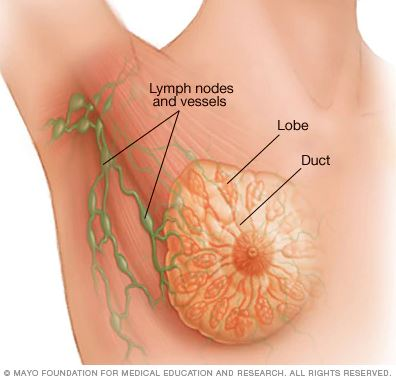
\includegraphics[width=0.75\textwidth]{Graphics/breast.jpg}
    \caption{Schematic of the female breast. The lobes form the milk producing system of the breast whereas the ducts are channels for the milk towards the nipple of the breast. Picture source: \cite{mayo-clinic}. }
    \label{anatomy_breast}
\end{figure}

\hspace{-1cm}
   
For the regular mammographic screenings typically X-ray-based imaging techniques are in use. The breasts has to be compressed between two plates so that a higher resolution of the breast tissue can be archived (see figure \ref{mammo_example_picture}). Besides the advantages of delivering results shortly after the screening and by having a high enough resolution to detect small tumour cells before they are detectable by palpation, there are certain downsides that have to be considered.
The biggest problem with X-ray-based mammographic screenings is the usage of ionising radiation. When it comes to x-ray and gamma radiation there is no such thing as a safe dose. Every dose of ionizing radiation of for example a low-dose X-ray mammography has proven to add to the incidence of breast cancer  \cite{Pauwels2015BreastRadiobiology} and so the main objective is the reduction of exposure to ionizing radiation.

\begin{figure}[H]
    \centering
    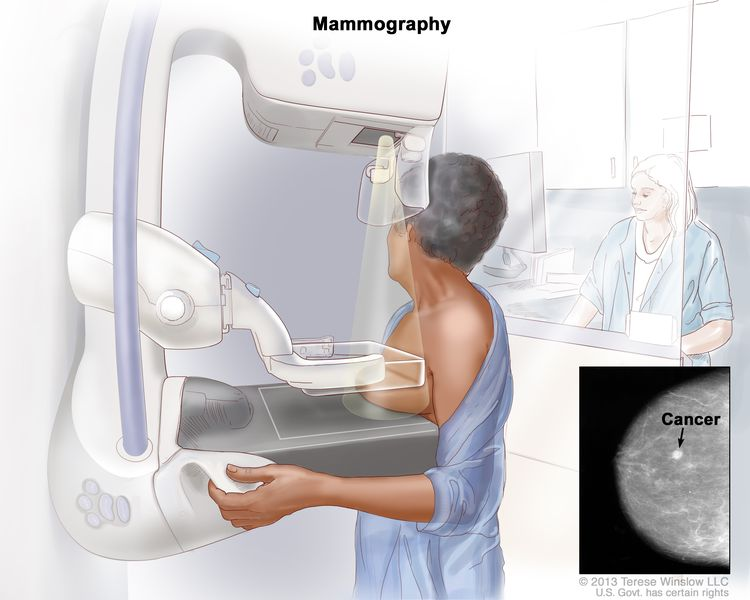
\includegraphics[width=0.75\textwidth]{mammography.jpg}
    \caption{Schematic of the mammography procedure. The breast is pressed between two plates and a beam of X-Ray-Radiation is used to produce the picture. On the bottom right is an example image of a female breast with the white dot indicating cancerogenous tissue. Picture source: \cite{NationalInstitutesofHealthNIH-NationalCancerInstituteNCIBreastTreatment}. }
    \label{mammo_example_picture}
\end{figure}

Another screening method is the physical examination of the breast either by the patient herself or during a clinical breast exam performed by a health professional. For this method the breast is carfully palpated to look for lumps or any kind of anomaly that might indicate an early stage of breast cancer. This method has one mayor disadvantage: lumps can only be detected by palpation after they have reached a certain size which, compared to the size of detectability during a mammography screening, is relatively large. Thus, the potential diagnosis of breast cancer solely by palpation often leads to the identification of first cancer symptoms in a later stage compared to mammography or \ac{usct} screening.   


Compared to the widely used X-ray-based screening method which uses ionizing radiation the three dimensional \ac{usct} has its advantages and makes this novel imaging technique a promising alternative to classical mammography. By utilizing the ultrasound echo technique high resolution 3D image of the breast tissue can be yielded without the use of ionizing radiation. Furthermore, the examination process with an \ac{usct} is much more comfortable for the patient since the breast does not have to be deformed during the imaging procedure. 




The total mastectomy is one of the possibilities to treat breast cancer. During this procedure big parts of the breast tissue as well as parts of the lymphatic system near the armpit are surgically removed (figure \ref{mastecto_example_picture}).  


\begin{figure}[H]
    \centering
    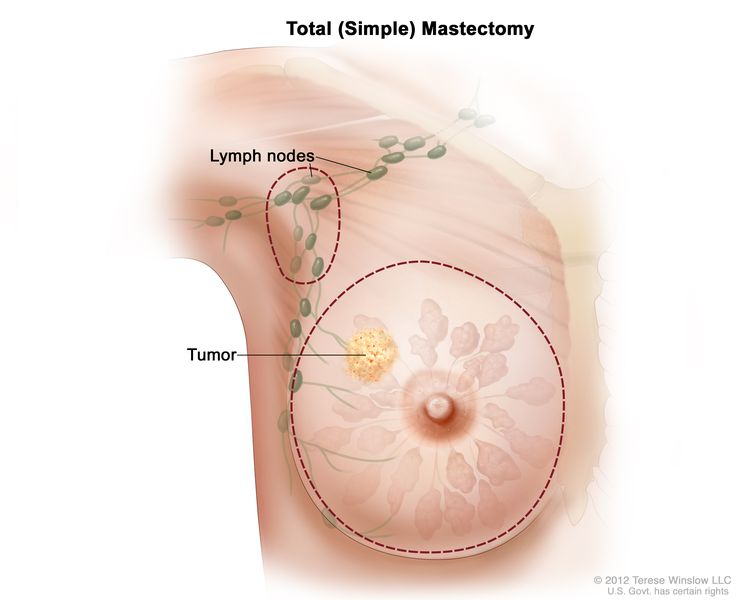
\includegraphics[width=0.75\textwidth]{Graphics/Mastectomy.jpg}
    \caption{Treatment of female breast cancer. During the mastectomy big parts of the breast are surgically removed (marked by dotted line). Picture source: \cite{NationalInstitutesofHealthNIH-NationalCancerInstituteNCIBreastTreatment}. }
    \label{mastecto_example_picture}
\end{figure}

This treatment may be combined with chemo therapy to decrease the size the tumour prior to the surgery. The post operative therapy often consists of radiation and hormone therapy to remove any cancer cells that might be left after the the mastectomy \cite{NationalInstitutesofHealthNIH-NationalCancerInstituteNCIBreastTreatment}.


\section{Motivation}

The goal of this thesis was to introduce a fourth modality to the reconstruction algorithm to further increase the resolution of the image as well as to classify different tissue types by analysing the back scattering. It is assumed that the tumour tissue consists of an inhomogeneous distribution of cancer cells which results in a distinct back scattering behaviour of the tissue.
By introducing the reflection characteristic algorithm to the reconstruction algorithm with an already implemented \ac{sos}-correction it is expected to further increase the clinical value of the reconstructed images as well as to make an assessment of the required computation power needed for the vast amount of data processing.


